\documentclass[Main]{subfiles}
\begin{document}

\section{Deployment View}
Systemet er bygget op af en fjernbetjening, dronen, samt modtagerenheden på dronen, vist på Figur \ref{Fig:DeploymentViewOverview}.

\begin{figure}[H]
\centering
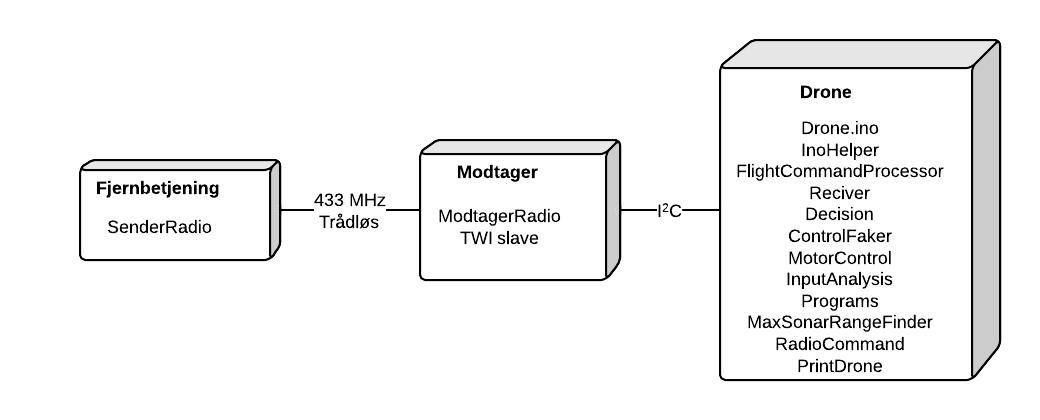
\includegraphics[width = 0.70 \textwidth]{DeploymentViewOverview}
\caption{Deployment View diagram}
\label{Fig:DeploymentViewOverview}
\end{figure}

Fjernbetjeningen sender sine signaler til dronen vha. det trådløse 433 MHz-signal, som opfanges af modtager-enheden.
Herefter sættes signalets værdi til rådighed, således dronen kan læse det igennem \itoc -forbindelsen.



\subsection{Protokoller}
En kort beskrivelse af protokollerne mellem de forskellige enheder.




\subsubsection{Fjernbetjening til modtager}

\begin{wrapfigure}{r}{0.5\textwidth}
  \centering
	\begin{tabular}{l l}
	\hline
	\textbf{Kommando} 	& \textbf{Indhold i bytes} \\ \hline
	Let 				& \code{0x3F} + \code{0x02} \\
	Autoland 			& \code{0x3F} + \code{0x04} \\
	Fremad 				& \code{0x3F} + \code{0x08} \\
	Roter til højre 	& \code{0x3F} + \code{0x0A} \\
	Roter til venstre 	& \code{0x3F} + \code{0x0C} \\
	Roter til højre 	& \code{0x3F} + \code{0x0E} \\
	Stop 				& \code{0x3F} + \code{0x10} \\
	Inkrementer højde 	& \code{0x3F} + \code{0x12} \\
	Dekrementer højde 	& \code{0x3F} + \code{0x14} \\ \hline	
  	\end{tabular}
  \makeatletter\def\@captype{table}\makeatother% "Change float to table"
  
\caption{Kommandoer sendt fra fjernbetjeningen}
\label{Tab:kommandoer}

\end{wrapfigure}

Ved tryk på knapperne på fjernbetjeningen sendes en frame til modtageren.
Signalet består af 2 bytes, hvoraf det første er en programindikator og den anden er selve programmet.

%Desværre står det sidste bit og svinger, hvilket kan være ganske kritisk for, hvilket program der bliver kørt og af den årsag shift'es alle bit én plads op i den sidste byte før forsendelse og én bit ned ved modtagelse.
%Dette giver mulighed for at sende $2^7 = 128$ programmer til eksekvering.

%Derudover kan det første byte indeholde forskellige indikatorer, hvilket giver mulighed for 256 forskellige typer beskeder, der hver indeholder 128 forskellige værdier.

Kommandoer der kan sendes vises i Tabel \ref{Tab:kommandoer}.



\subsubsection{Modtager til drone}
Når en frame er modtaget på modtagerradioen, tjekker den framen for om CRC passe. Hvis der er uoverensstemmelse, melle størrelsen på frame og CRC verdien, bliver framen kasseret. Hvis framens størrelse og CRC stemmer overens, laver modtagerradioen et interrupt på microcontroller 2. Microcontrolleren vil så hente den modtaget pakke fra radioen, strippe den for pakke længde. Hverefter vil den blive lagt ud i en output buffer til I2C forbindelsen til dronen. Som så kan hente den næste gang den har tid. 



\end{document}